\section{Training language models}
\subsection{Model Comparison}
In this section we will present the result of the first experiment of the 3 models, that is vanilla RNN, GRU, and Transformer, with respectively the correspondant given hyperparameters shown in Table~\ref{table:1}. We run these model for the same number of epochs which is 40.
	\begin{table}[H]
		\centering
		\begin{tabular}{||c c c c||} 
			\hline
			    \textbf{Hyperparameters} & \textbf{Vanilla RNN} & \textbf{RNN with GRU }& \textbf{Transformer} \\[0.5ex] 
			\hline
			Optimizer & ADAM & SGD\_LR\_SCHEDULE & SGD\_LR\_SCHEDULE\\
			Learning rate & 0.0001 & 10 & 20 \\
			Batch size & 20 &20 &  128 \\
			Sequence length & 35 & 35 & 35\\
			Hidden size & 1500 & 1500 & 512\\
			Number of layers & 2 & 2 & 6\\
			Dropout probability & 0.35 &0.35  & 0.9\\[1ex]
	\hline
		\end{tabular}
		\caption{Model's settings}
		\label{table:1}
	\end{table}
	
	The table~\ref{table:2} show the result of this first experiment. We notice that the Transformer is the best model in terms of time-processus and validation/training loss. The GRU is the most expensive model in term of time processing but gives a better result than the vanilla RNN. The latter is the worst one in term of training and validation loss.
	
	\begin{table}[H]
		\centering
		\begin{tabular}{||c c c c||} 
			\hline
			\textbf{Result} & \textbf{Vanilla RNN} & \textbf{RNN with GRU }& \textbf{Transformer} \\[0.5ex] 
			\hline
			Training PPL & 120.97 & 65.85 & ???\\
			Validation PPL & 157.82 & 102.63 & ??? \\
			Time processing per epoch (s) & 411.05 & 668.06 & 174.59\\[1ex]
			\hline
		\end{tabular}
		\caption{First experiment results}
		\label{table:2}
	\end{table}

This result are pretty close to the expected perplexities given as reference:
\begin{itemize}
	\item[-] RNN: train:  120  val: 157
	\item[-] GRU: train:   65  val: 104
	\item[-] TRANSFORMER:  train:  67  val: 146
\end{itemize}

Which proves that our models are well implemented!

Lastly, the Figures below show the learning curves for (train and validation) PPL per epoch and per wall-clock-time, for respectively the architectures above:

\begin{figure}[H]
	\centering
	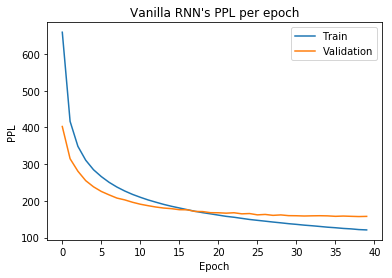
\includegraphics[scale=0.8]{VRNN_LC_EPOCH.png}
	\caption{Vanilla RNN's PPL per epoch}
	\label{fig:fig1}
\end{figure}

\begin{figure}[H]
	\centering
	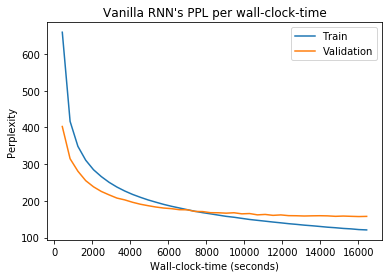
\includegraphics[scale=0.8]{VRNN_LC_TIME.png}
	\caption{Vanilla RNN's PPL per wall-clock-time}
	\label{fig:fig2}
\end{figure}

\begin{figure}[H]
	\centering
	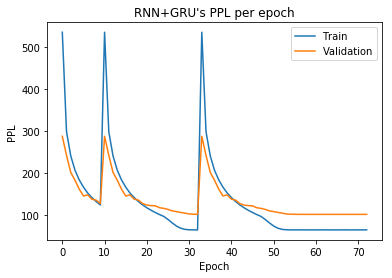
\includegraphics[scale=0.8]{GRU_LC_EPOCH.png}
	\caption{RNN with GRU PPL per epoch}
	\label{fig:fig3}
\end{figure}

\begin{figure}[H]
	\centering
	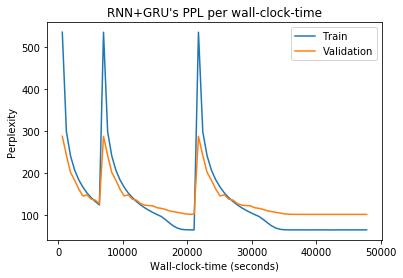
\includegraphics[scale=0.8]{GRU_LC_TIME.png}
	\caption{RNN with GRU PPL per wall-clock-time}
	\label{fig:fig4}
\end{figure}


\subsection{Exploration of optimizers}
In this section we will explore different optimizers for each of the previous models, along with some changes in the hyperparameters such as learning rate or hidden size or number of layers. We assume that those changes on the hyperparameters give a fair baseline to compare reasonably the effect of each optimizer on our 3 models. We kept the hyperparameters of experiment 1 for comparison matters.

I\textcolor{red}{nclude the following tables:
	1. For each experiment in 1-3, plot learning curves (train and validation) of PPL over both
	epochs and wall-clock-time.}

\begin{itemize}
	\item[1)] \textbf{Results for Vanilla RNN:}
	The hyperparameters used for experiments 2 and 3 are given in the Table~\ref{table:3}.\\
	\begin{table}[H]
		\centering
		\begin{tabular}{||c c c c||} 
			\hline
			\textbf{Hyperparameters} & \textbf{Experiment 1} &\textbf{Experiment 2} & \textbf{Experiment 3}\\[0.5ex] 
			\hline
			Optimizer & ADAM & SGD & SGD\_LR\_SCHEDULE \\
			Learning rate & 0.0001 & 0.0001 & 1  \\
			Batch size &20 & 20 &20 \\
			Sequence length &35 & 35 & 35\\
			Hidden size & 1500 & 1500 & 512 \\
			Number of layers & 2 & 2 & 2 \\
			Dropout probability & 0.35 & 0.35 &0.35 \\[1ex]
			\hline
		\end{tabular}
		\caption{Vanilla RNN additionnal experiments' hyperparameters}
		\label{table:3}
	\end{table}
	%
	The results of these experiments are shown in the Table~\ref{table:3.1}. We notice that the SGD got the worse result and it couldn't converge within 40 epochs, wheras ADAM gets the best result for the same number of epochs and the same hyperparameters. Additionnaly, the SGD\_LR\_SCHEDULE works better than SGD for a bigger learning rate and lower capacity of the model. We can conclude that ADAM is the better optimizer for vanilla RNN given the hyperparameters shown at Table~\ref{table:3}.
	\begin{table}[H]
		\centering
		\begin{tabular}{||c c c c||} 
			\hline
			\textbf{Result} & \textbf{Experiment 1} & \textbf{Experiment 2}& \textbf{Experiment 3} \\[0.5ex] 
			\hline
			Training PPL & 120.97 & 3008.63 & 229.56 \\
			Validation PPL & 157.82 & 2220.49 & 195.67  \\
			Average time processing per epoch (s) & 411 & 384 & 185 \\[1ex]
			\hline
		\end{tabular}
		\caption{Vanilla RNN results experiments}
		\label{table:3.1}
	\end{table}
	%
	\item[2)] \textbf{Results for RNN with GRU:}
	The experiments 2 and 3, for RNN with GRU model, used respectively the parameters given in Table~\ref{table:4}.\\
	%
	\begin{table}[H]
		\centering
		\begin{tabular}{||c c c c||} 
			\hline
			\textbf{Hyperparameters} &\textbf{Experiment 1} & \textbf{Experiment 2} & \textbf{Experiment 3}\\[0.5ex] 
			\hline
			Optimizer & SGD\_LR\_SCHEDULE & SGD & ADAM \\
			Learning rate & 10 & 10 & 0.0001   \\
			Batch size & 20 & 20 &20 \\
			Sequence length & 35 & 35 & 35\\
			Hidden size & 1500 & 1500 & 1500 \\
			Number of layers & 2 & 2 & 2 \\
			Dropout probability & 0.35 & 0.35 &0.35 \\[1ex]
			\hline
		\end{tabular}
		\caption{RNN with GRU additionnal experiments' hyperparameters}
		\label{table:4}
	\end{table}
	%
	The results are shown in Table~\ref{table:4.1}. We notice that SGD\_LR\_SCHEDULE did the best result on the validation set but the worst in training set, which means he generalize well and has lowest variance. The SGD did a better result than with the Vanilla RNN experiment due to a bigger learning rate, which is logic as he must make bigger steps within a limited number of epochs. ADAM did the best job on the training set, but the variance was greater than SGD\_LR\_SCHEDULE, which may seem as a beggining of overfitting.
	\begin{table}[H]
		\centering
		\begin{tabular}{||c c c c||} 
			\hline
			\textbf{Result} & \textbf{Experiment 1} & \textbf{Experiment 2}& \textbf{Experiment 3} \\[0.5ex] 
			\hline
			Training PPL & 65.85& 50.33& 59.98 \\
			Validation PPL & 102.63 & 121.36 & 113.71  \\
			Average time processing per epoch (s) & 668 & 648 & 675 \\[1ex]
			\hline
		\end{tabular}
		\caption{First experiment results}
		\label{table:4.1}
	\end{table}
	%
		\item[3)] \textbf{Results for Transformer:}
		And finally the Transformer used the following parameters:
		%
		\begin{table}[H]
			\centering
			\begin{tabular}{||c c c c||} 
				\hline
				\textbf{Hyperparameters} &\textbf{Experiment 1} & \textbf{Experiment 2} & \textbf{Experiment 3}\\[0.5ex] 
				\hline
				Optimizer & SGD\_LR\_SCHEDULE & SGD & ADAM\\
				Learning rate & 20 & 20 & 0.001  \\
				Batch size & 128 & 128 & 128 \\
				Sequence length & 35 & 35 & 35\\
				Hidden size & 512 & 512 & 512 \\
				Number of layers & 6 & 6 & 2 \\
				Dropout probability & 0.9 & 0.9 &0.9 \\[1ex]
				\hline
			\end{tabular}
			\caption{Transformer additionnal experiments' hyperparameters}
			\label{table:5}
		\end{table}
And gives the following results:
%
The Transformer got the following results:
\begin{table}[H]
	\centering
	\begin{tabular}{||c c c c||} 
		\hline
		\textbf{Result} & \textbf{Experiment 1} & \textbf{Experiment 2}& \textbf{Experiment 3} \\[0.5ex] 
		\hline
		Training PPL & ??? & ??? & ???  \\
		Validation PPL & ???  & ???  & ???  \\
		Average time processing per epoch (s) & ???  & ???  & ???  \\[1ex]
		\hline
	\end{tabular}
	\caption{First experiment results}
	\label{table:5.1}
\end{table}
\end{itemize}
%
As a global conclusion, and assuming that the comparison here was made with a set of hyperparameters that give a fair baseline for all the models, we can say that there is no universal best optimizer regardeless of the model architecture. In fact, each model architecture works better with a suited optimizer. Howerver, we notice that ADAM is very powerfull optimizer that can makes the model converge very quickly and if not well tuned could makes the model overfitt the training data. For the next experiment we will use the best optimizer that gave the better result and we will do a hyperparameter to find the best parameters that gives a better result than those found in these experiments.



\subsection{Exploration of hyperparmeters}

\textcolor{red}{Figures and Tables:
Each table and gure should have an explanatory caption. 
For tables, this goes above, for figures it goes below. 
Tables should have appropriate column and/or row headers.
Figures should have labelled axes and a legend. }

I\textcolor{red}{nclude the following tables:
1. For each experiment in 1-3, plot learning curves (train and validation) of PPL over both
epochs and wall-clock-time.}

\textcolor{red}{2. Make a table of results summarizing the train and validation performace for each experiment,
	indicating the architecture and optimizer. Sort by architecture, then optimizer, and number
	the experiments to refer to them easily later. Bold the best result for each architecture.}

\textcolor{red}{3. List all of the hyperparameters for each experiment in your report (e.g. specify the command
you run in the terminal to launch the job, including the command line arguments).}

4. Make 2 plots for each optimizer; one which has all of the validation curves for that optimizer
over epochs and one over wall-clock-time.
5. Make 2 plots for each arcitecture; one which has all of the validation curves for that architecture
over epochs and one over wall-clock-time.
\subsection{Discussion}